\documentclass[11pt,a4paper]{article}

\usepackage[margin=2.1cm]{geometry}
\usepackage[T1]{fontenc}
\usepackage[utf8]{inputenc}
\usepackage{lmodern}
\usepackage{microtype}
\usepackage{amsmath,amssymb,mathtools}
\usepackage{booktabs,array,tabularx}
\usepackage{graphicx}
\usepackage{xcolor}
\usepackage{tcolorbox}
\tcbuselibrary{skins,breakable}
\usepackage{fancyhdr}
\usepackage{hyperref}
\usepackage{enumitem}

\definecolor{navy}{HTML}{1B365D}
\definecolor{slate}{HTML}{2C5282}
\definecolor{tint}{HTML}{F4F7FA}
\definecolor{amber}{HTML}{8A5A00}
\definecolor{ambertint}{HTML}{FFFBEB}
\definecolor{greenink}{HTML}{1E5631}
\definecolor{greentint}{HTML}{F1F8F4}

\hypersetup{
  colorlinks=true,
  linkcolor=slate,
  urlcolor=slate,
  pdftitle={Ice Growth from Nucleation to Macroscopic Solid Mass: Dimensional Closure, Simulation and Verification},
  pdfauthor={rosolver Scientific Study}
}

\pagestyle{fancy}
\fancyhf{}
\fancyhead[L]{\small\color{slate}\textsc{Ice Growth: Nucleation to Solid Mass (\texttt{rosolver})}}
\fancyhead[R]{\small\color{slate}Dimensional Audit $\cdot$ Eq.~(16) $\cdot$ ODE/Stefan V\&V}
\fancyfoot[C]{\small\thepage}
\renewcommand{\headrulewidth}{0.4pt}

\newtcolorbox{setupbox}[1]{
  breakable, enhanced, colback=tint, colframe=navy, boxrule=0.8pt, arc=3pt,
  left=8pt, right=8pt, top=6pt, bottom=6pt, fonttitle=\bfseries\color{white}, title={#1}
}
\newtcolorbox{insightbox}[1]{
  breakable, enhanced, colback=ambertint, colframe=amber, boxrule=0.8pt, arc=3pt,
  left=8pt, right=8pt, top=6pt, bottom=6pt, fonttitle=\bfseries\color{white}, title={#1}
}
\newtcolorbox{resultbox}[1]{
  breakable, enhanced, colback=greentint, colframe=greenink, boxrule=0.8pt, arc=3pt,
  left=8pt, right=8pt, top=6pt, bottom=6pt, fonttitle=\bfseries\color{white}, title={#1}
}

\newcommand{\dd}{\mathrm{d}}
\newcommand{\pd}[2]{\frac{\partial #1}{\partial #2}}
\newcommand{\td}[2]{\frac{\dd #1}{\dd #2}}
\newcommand{\dimbr}[1]{\left[#1\right]}

\title{
  {\color{navy}\rule{\textwidth}{1.8pt}}\\[0.6em]
  {\LARGE\bfseries\color{navy} Modeling Ice Growth from Nucleation to Macroscopic Solid Mass}\\[0.35em]
  {\large\color{slate} Dimensional Audit of Eq.~(16), Exact Analytical Closure, Coupled ODE/\texttt{Stefan1D} Simulation \& V\&V}\\[0.4em]
  {\color{navy}\rule{\textwidth}{0.8pt}}
}
\author{Technical Study \& Lecture Notes\\[2pt]{\small\texttt{python -m examples.ice\_nucleation\_growth\_study.run\_study}}}
\date{\today}

\begin{document}
\maketitle

\begin{abstract}
\noindent We present a rigorous physical explanation, dimensional audit, analytical solution, numerical simulation, and verification study of the multi-scale ice growth formulation linking volumetric nucleation ($\partial_t N = \beta$), variable-mass crystal growth ($N\partial_t m + m\partial_t N$), macroscopic growth-front advancement ($m = \rho\sigma z$), and 1D Euler pressure-gradient balance ($\partial_t^2 z = -\frac{1}{\sigma\rho}\ddot{m}_{\mathrm{opp}} = -\frac{1}{\rho}\partial_z p$, Eq.~16). Resolving three latent normalization and geometric shortcuts in the draft equations produces a dimensionally exact 6-state ODE system admitting closed-form algebraic solutions ($z(t) = z_{\max} - (z_{\max}-z_0)N_0/(N_0+\beta t)$, $\dot{z}\propto t^{-2}$, $\partial_z p \propto t^{-3}$) and two exact symbolic conservation invariants (mass $m + m_{\mathrm{liq}} = m_{\max}$ and Eq.~16 momentum-impulse $\rho\dot{z} + \int_0^t \partial_z p\,\dd\tau = \rho\dot{z}_0$). Numerical simulations in \texttt{rosolver} achieve $\max|z_{\mathrm{RK4}} - z_{\mathrm{exact}}| = 1.68\times 10^{-11}\text{ m}$, RK4 observed convergence order $p_{\mathrm{obs}} = 4.067$, dual conservation residuals $\le 2.11\times 10^{-15}$, and a direct comparison against continuum moving-boundary \texttt{Stefan1D} freezing.
\end{abstract}

\tableofcontents
\vspace{0.8em}
\hrule
\vspace{1em}

% ============================================================================
\section{Physical Explanation \& Step-by-Step Dimensional Audit}
% ============================================================================

\begin{setupbox}{Original Draft Equations Under Review}
\begin{align*}
  \pd{N}{t} &= \beta,
  & N\pd{m}{t} + m\pd{N}{t},
  & \qquad N\pd{(\rho V)}{t} = \beta(1 - \rho V),\\
  \rho\sigma\pd{z}{t} &= n(1 - \rho\dot{V}),
  & \pd{^2 z}{t^2} &= -\frac{1}{\sigma\rho}\ddot{m} = -\frac{1}{\rho}\pd{p}{z} \qquad\text{(Eq.~16)}.
\end{align*}
\end{setupbox}

\subsection{The 3-Stage Physical Narrative}
\begin{enumerate}[leftmargin=1.5em,itemsep=3pt]
  \item \textbf{Stage 1 — Discrete Nucleation ($\pd{N}{t} = \beta$)}: Ice nuclei appear in supercooled liquid at volumetric nucleation rate $\beta$ ($\dimbr{\beta} = \mathsf{L}^{-3}\mathsf{T}^{-1}$), raising particle number density $N(t) = N_0 + \beta t$ ($\dimbr{N} = \mathsf{L}^{-3}$).
  \item \textbf{Stage 2 — Variable-Mass Crystal Growth ($\pd{(Nm)}{t} = N\pd{m}{t} + m\pd{N}{t}$)}: Total solid ice mass per unit system volume $M = N m$ grows both by \emph{accretion onto existing crystals} ($N\dot{m}$) and by \emph{nucleation of new particles} ($m\beta$). Setting total rate to a reservoir-limited ceiling $\beta m_{\max}$ yields self-limiting crystal growth $N\dot{m} = \beta(m_{\max} - m)$.
  \item \textbf{Stage 3 — Macroscopic Solid Front \& Eq.~(16) Momentum Balance}: With constant solid ice density $\rho = 917\text{ kg/m}^3$ and 1D slab volume $V = \sigma z$ ($\sigma = A$, cross-sectional area), crystal growth maps directly onto macroscopic front length $z(t)$. Differentiating once more gives front deceleration $\ddot{z} < 0$, which equals the opposing crystallization/hydrostatic pressure gradient $-\frac{1}{\rho}\pd{p}{z}$ (1D Euler equation).
\end{enumerate}

\subsection{Dimensional Closure Fixes Required Before Simulation}
\begin{table}[htbp]
\centering
\caption{Dimensional and Algebraic Audit of Draft Equations}
\label{tab:audit}
\renewcommand{\arraystretch}{1.22}
\footnotesize
\begin{tabularx}{\textwidth}{@{}l l X@{}}
\toprule
\textbf{Draft Expression} & \textbf{Audit Finding} & \textbf{Dimensionally Exact Closure} \\
\midrule
$1 - \rho V$ & Mixes dimensionless $1$ with mass $\rho V$ ($\mathsf{M}$) & Replace $1 \to m_{\max} = \rho\sigma z_{\max}$ (reservoir mass cap, $\mathsf{M}$) \\
$\sigma = A\,\dd z$ & Yields $\dimbr{\sigma}=\mathsf{L}^3$, breaking $\dimbr{\rho\sigma\dot{z}}=\mathsf{M}\mathsf{T}^{-1}$ & Define cross-sectional area $\sigma = A$ ($\mathsf{L}^2$), so $\dd V = \sigma\,\dd z$ \\
$n(1 - \rho\dot{V})$ & Mixes $V$ with $\dot{V}$ and drops $V_{\mathrm{sys}}^{-1}$ & Use exact coupled rate $\rho\sigma\dot{z} = \frac{\beta}{N}(m_{\max} - \rho\sigma z)$ \\
$-\frac{1}{\sigma\rho}\ddot{m} = -\frac{1}{\rho}\pd{p}{z}$ & Dimensionally exact ($\mathsf{L}\mathsf{T}^{-2}$); sign reflects opposing deceleration & $\ddot{z} = -2\frac{\beta}{N}\dot{z} = -\frac{1}{\rho}\pd{p}{z}$ with $\pd{p}{z} > 0$ opposing front growth \\
\bottomrule
\end{tabularx}
\end{table}

% ============================================================================
\section{Exact Analytical Solution \& Conservation Invariants}
% ============================================================================

For constant nucleation rate $\beta > 0$, initial seed concentration $N_0 > 0$, and $m = \rho\sigma z$ ($z_{\max} = m_{\max}/(\rho\sigma)$), the closed system is separable:
\begin{equation}
  \frac{\dd z}{z_{\max} - z} = \frac{\beta\,\dd t}{N_0 + \beta t}
  \quad\Longrightarrow\quad
  z(t) = z_{\max} - (z_{\max} - z_0)\frac{N_0}{N_0 + \beta t}.
  \label{eq:z_exact}
\end{equation}
Differentiating Eq.~\eqref{eq:z_exact} twice yields the exact front velocity, deceleration, and Eq.~(16) crystallization pressure gradient:
\begin{align}
  \dot{z}(t) &= \frac{(z_{\max} - z_0)N_0\beta}{(N_0 + \beta t)^2},
  \qquad
  \ddot{z}(t) = -\frac{2(z_{\max} - z_0)N_0\beta^2}{(N_0 + \beta t)^3},\\
  \pd{p}{z}(t) &= -\rho\,\ddot{z}(t) = \frac{2\rho(z_{\max}-z_0)N_0\beta^2}{(N_0 + \beta t)^3} > 0.
  \label{eq:kinematics_exact}
\end{align}
Notice that $\ddot{z}(t) = -2(\beta/N)\dot{z}(t)$, giving a closed second-order dynamical equation whose asymptotic late-time scaling is $\dot{z} \propto t^{-2}$ and $\partial_z p \propto t^{-3}$.

\begin{insightbox}{Two Exact Symbolic Conservation Laws}
Introducing remaining supercooled liquid mass $m_{\mathrm{liq}}(t)$ and time-integrated pressure gradient $P_{\mathrm{imp}}(t) = \int_0^t \pd{p}{z}(\tau)\,\dd\tau$, the 6-state ODE system obeys two exact invariants:
\begin{equation}
  \td{}{t}\bigl(m + m_{\mathrm{liq}}\bigr) \equiv 0 \quad (\text{Mass}),
  \qquad\qquad
  \td{}{t}\bigl(\rho\dot{z} + P_{\mathrm{imp}}\bigr) \equiv 0 \quad (\text{Eq.~16 Momentum-Impulse}).
\end{equation}
\end{insightbox}

% ============================================================================
\section{Simulation Results \& Visual Analysis}
% ============================================================================

We simulate a $50\text{ mm}$ freezing slab ($\sigma = 0.01\text{ m}^2$, $\rho = 917\text{ kg/m}^3$, $m_{\max} = 0.4585\text{ kg}$, $N_0 = 10^4\text{ m}^{-3}$) across four nucleation regimes $\beta \in \{50, 200, 600, 1500\}\text{ m}^{-3}\text{s}^{-1}$ over $t \in [0, 600]\text{ s}$, detect random-close-packing coalescence ($\phi_c = z/z_{\max} = 0.64$) via \texttt{EventSpec}, and benchmark against continuum moving-boundary \texttt{Stefan1D} freezing ($T_{\mathrm{wall}} = -15^\circ\text{C}$, $\delta \propto \sqrt{t}$).

\begin{table}[htbp]
\centering
\caption{Simulated Nucleation Regimes ($\tau_N = N_0/\beta$, Coalescence $t_c$ at $\phi_c=0.64$, Solidification $t_{90}$)}
\label{tab:regimes}
\renewcommand{\arraystretch}{1.22}
\footnotesize
\begin{tabularx}{\textwidth}{@{}lccccc@{}}
\toprule
\textbf{Nucleation Regime} & $\beta$ [$\mathrm{m}^{-3}\mathrm{s}^{-1}$] & $\tau_N$ [s] & $t_c$ ($\phi=0.64$) [s] & $t_{90}$ [s] & $z(600\text{ s})$ [mm] \\
\midrule
Slow Nucleation & $50$ & $200.0$ & $350.0$ & $1780.0$ & $37.625$ \\
Reference Case & $200$ & $50.0$ & $87.5$ & $445.0$ & $46.192$ \\
Fast Nucleation & $600$ & $16.7$ & $29.2$ & $148.3$ & $48.662$ \\
Rapid Quench & $1500$ & $6.7$ & $11.7$ & $59.3$ & $49.456$ \\
\bottomrule
\end{tabularx}
\end{table}

\begin{figure}[htbp]
  \centering
  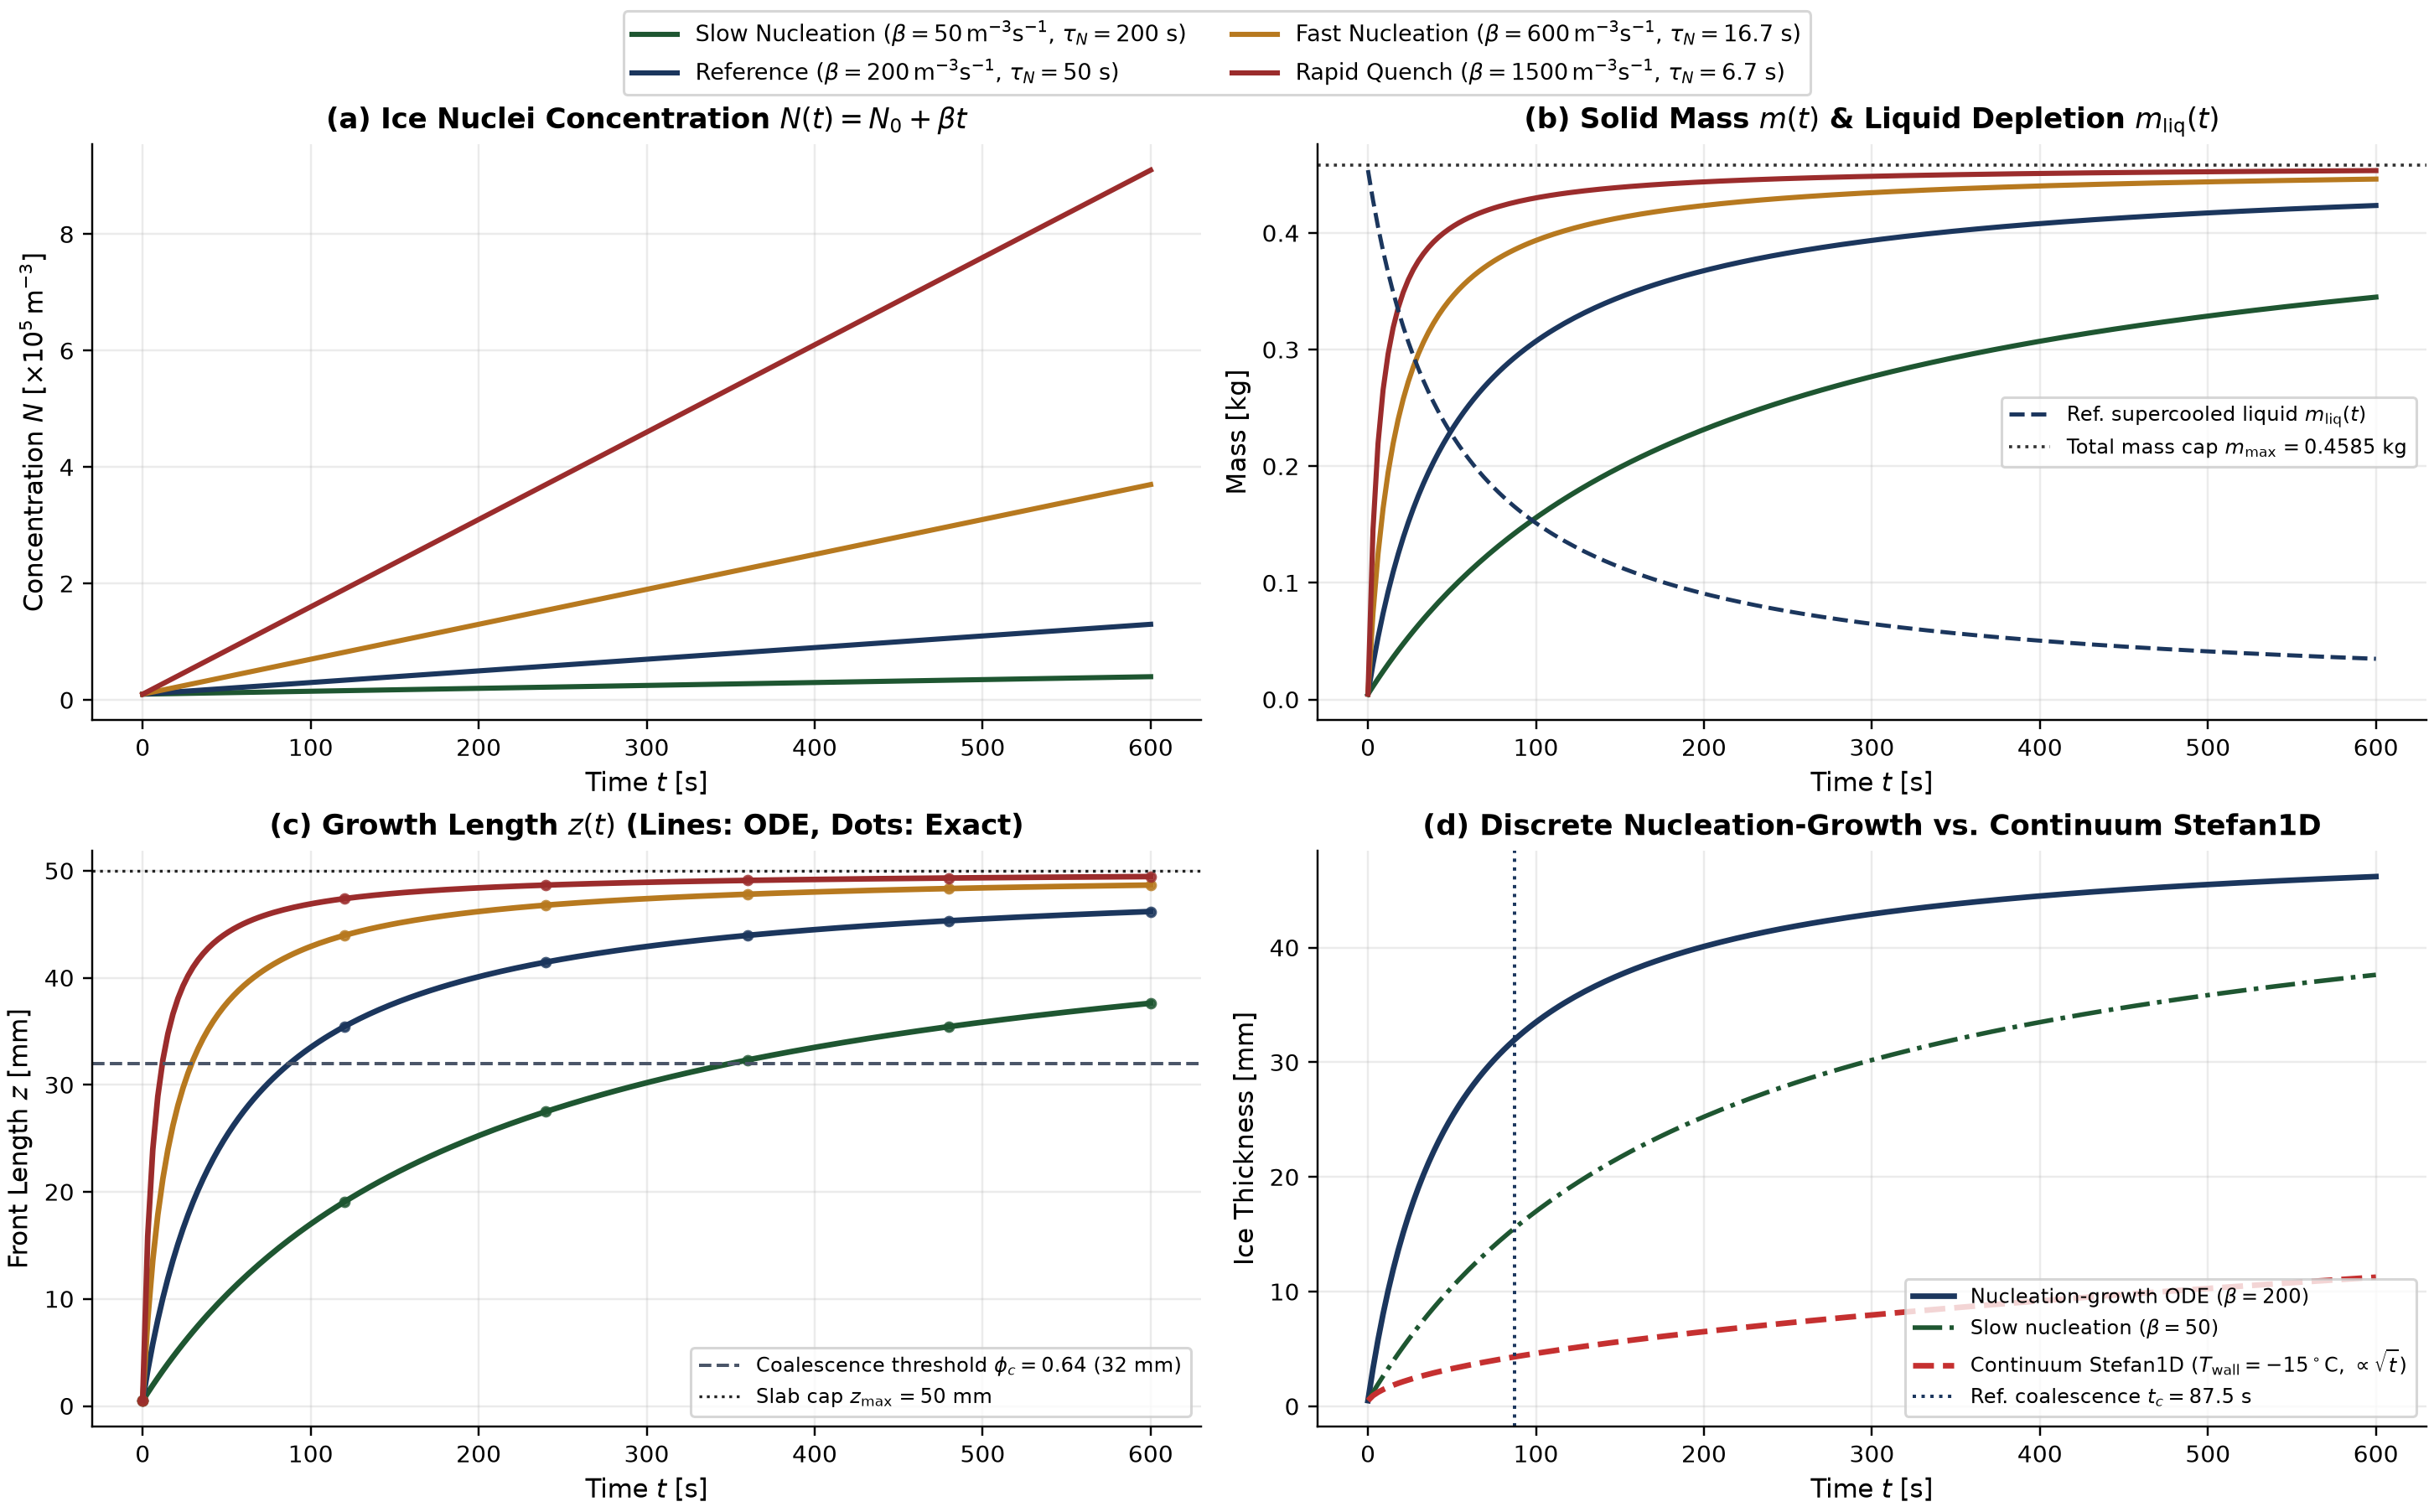
\includegraphics[width=0.98\textwidth]{../../figures/ice_fig1_multiscale_timeline.png}
  \caption{Multi-scale ice growth timeline: (a)~nuclei concentration $N(t)$, (b)~solid ice mass $m(t)$ and supercooled liquid depletion $m_{\mathrm{liq}}(t)$, (c)~macroscopic front length $z(t)$ comparing RK4 ODE (lines) with exact Eq.~\eqref{eq:z_exact} (dots), and (d)~nucleation-driven front vs.\ continuum thermal-conduction \texttt{Stefan1D} front ($\delta(600\text{ s}) = 11.26\text{ mm}$).}
  \label{fig:timeline}
\end{figure}

\begin{figure}[htbp]
  \centering
  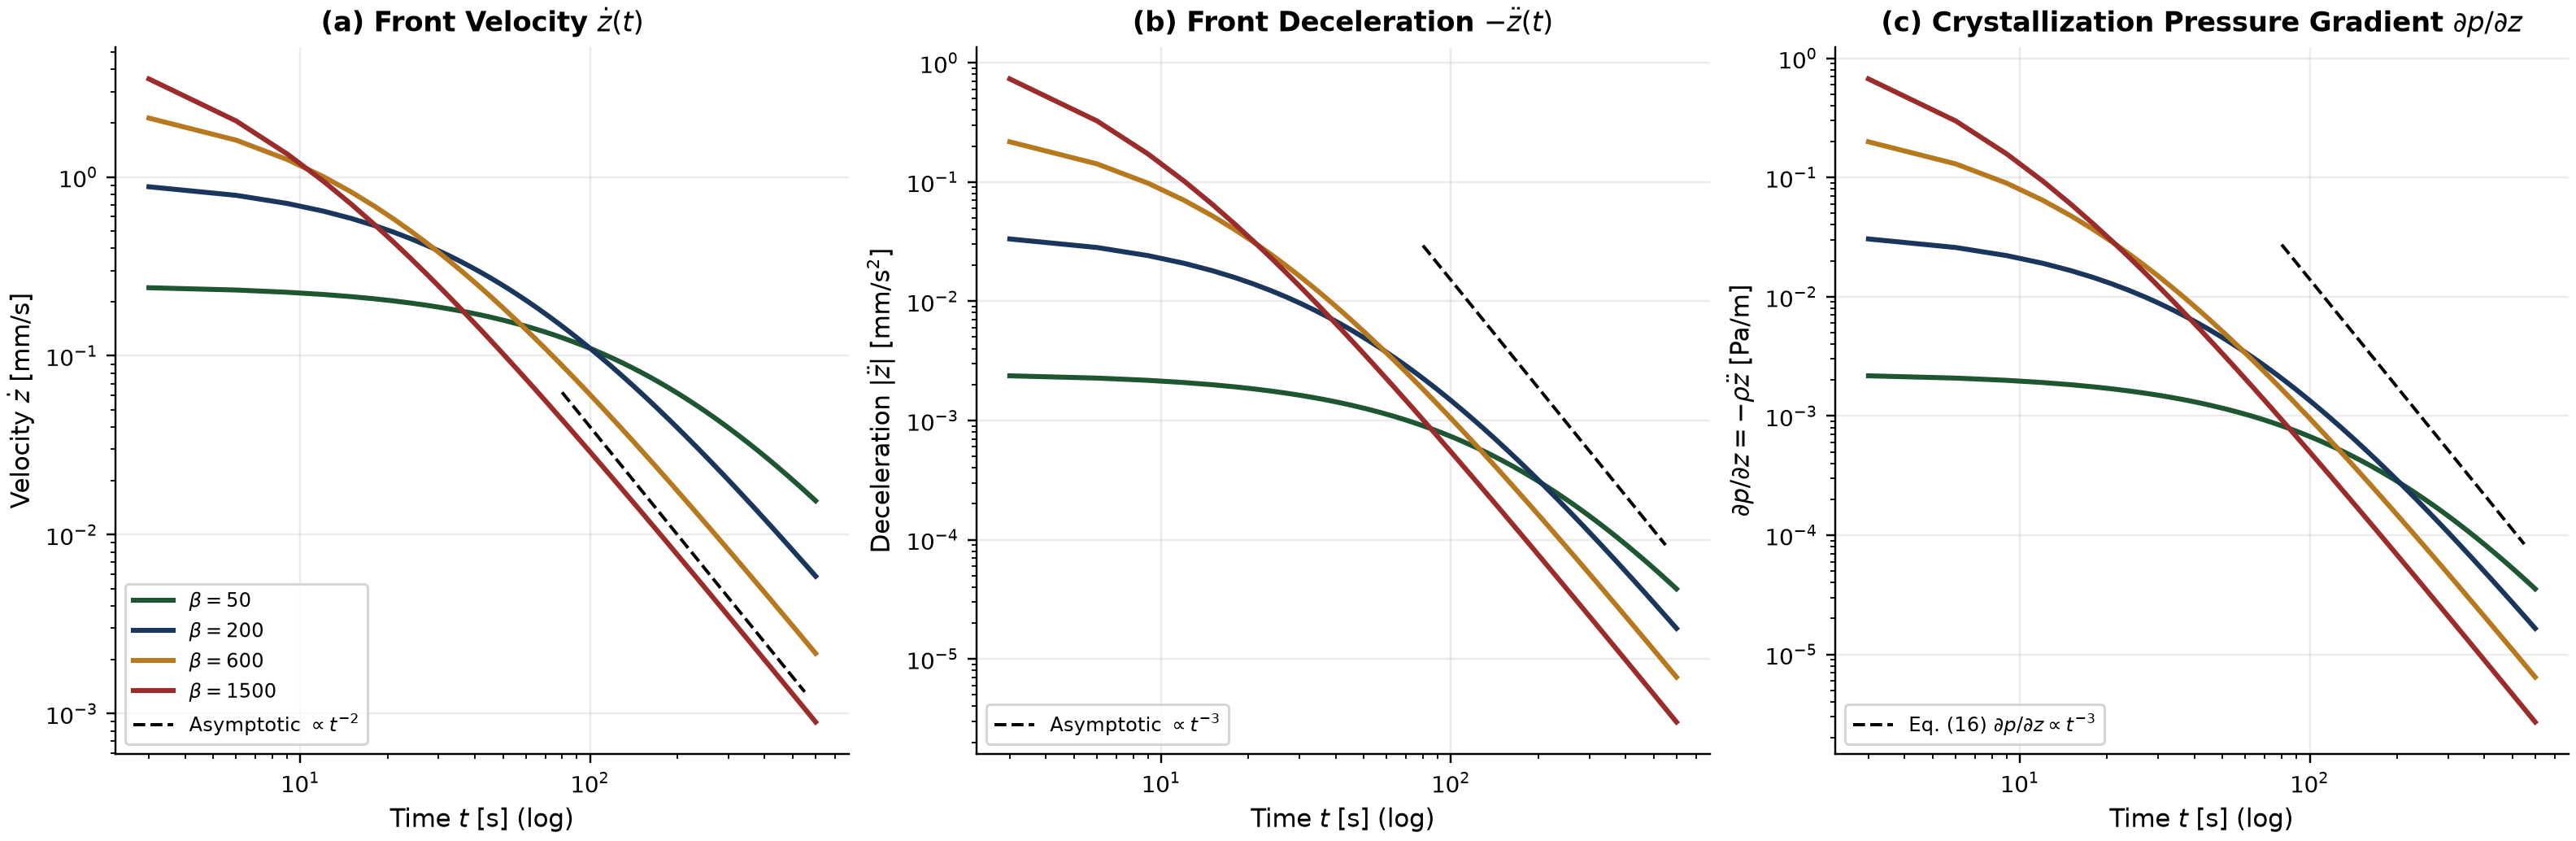
\includegraphics[width=0.98\textwidth]{../../figures/ice_fig2_kinematics_pressure.png}
  \caption{Log--log kinematics and Eq.~(16) pressure coupling: (a)~front velocity $\dot{z}(t)$ approaching $t^{-2}$, (b)~front deceleration $-\ddot{z}(t)$ approaching $t^{-3}$, and (c)~induced opposing crystallization pressure gradient $\partial_z p = -\rho\ddot{z}$ [Pa/m].}
  \label{fig:kinematics}
\end{figure}

\begin{figure}[htbp]
  \centering
  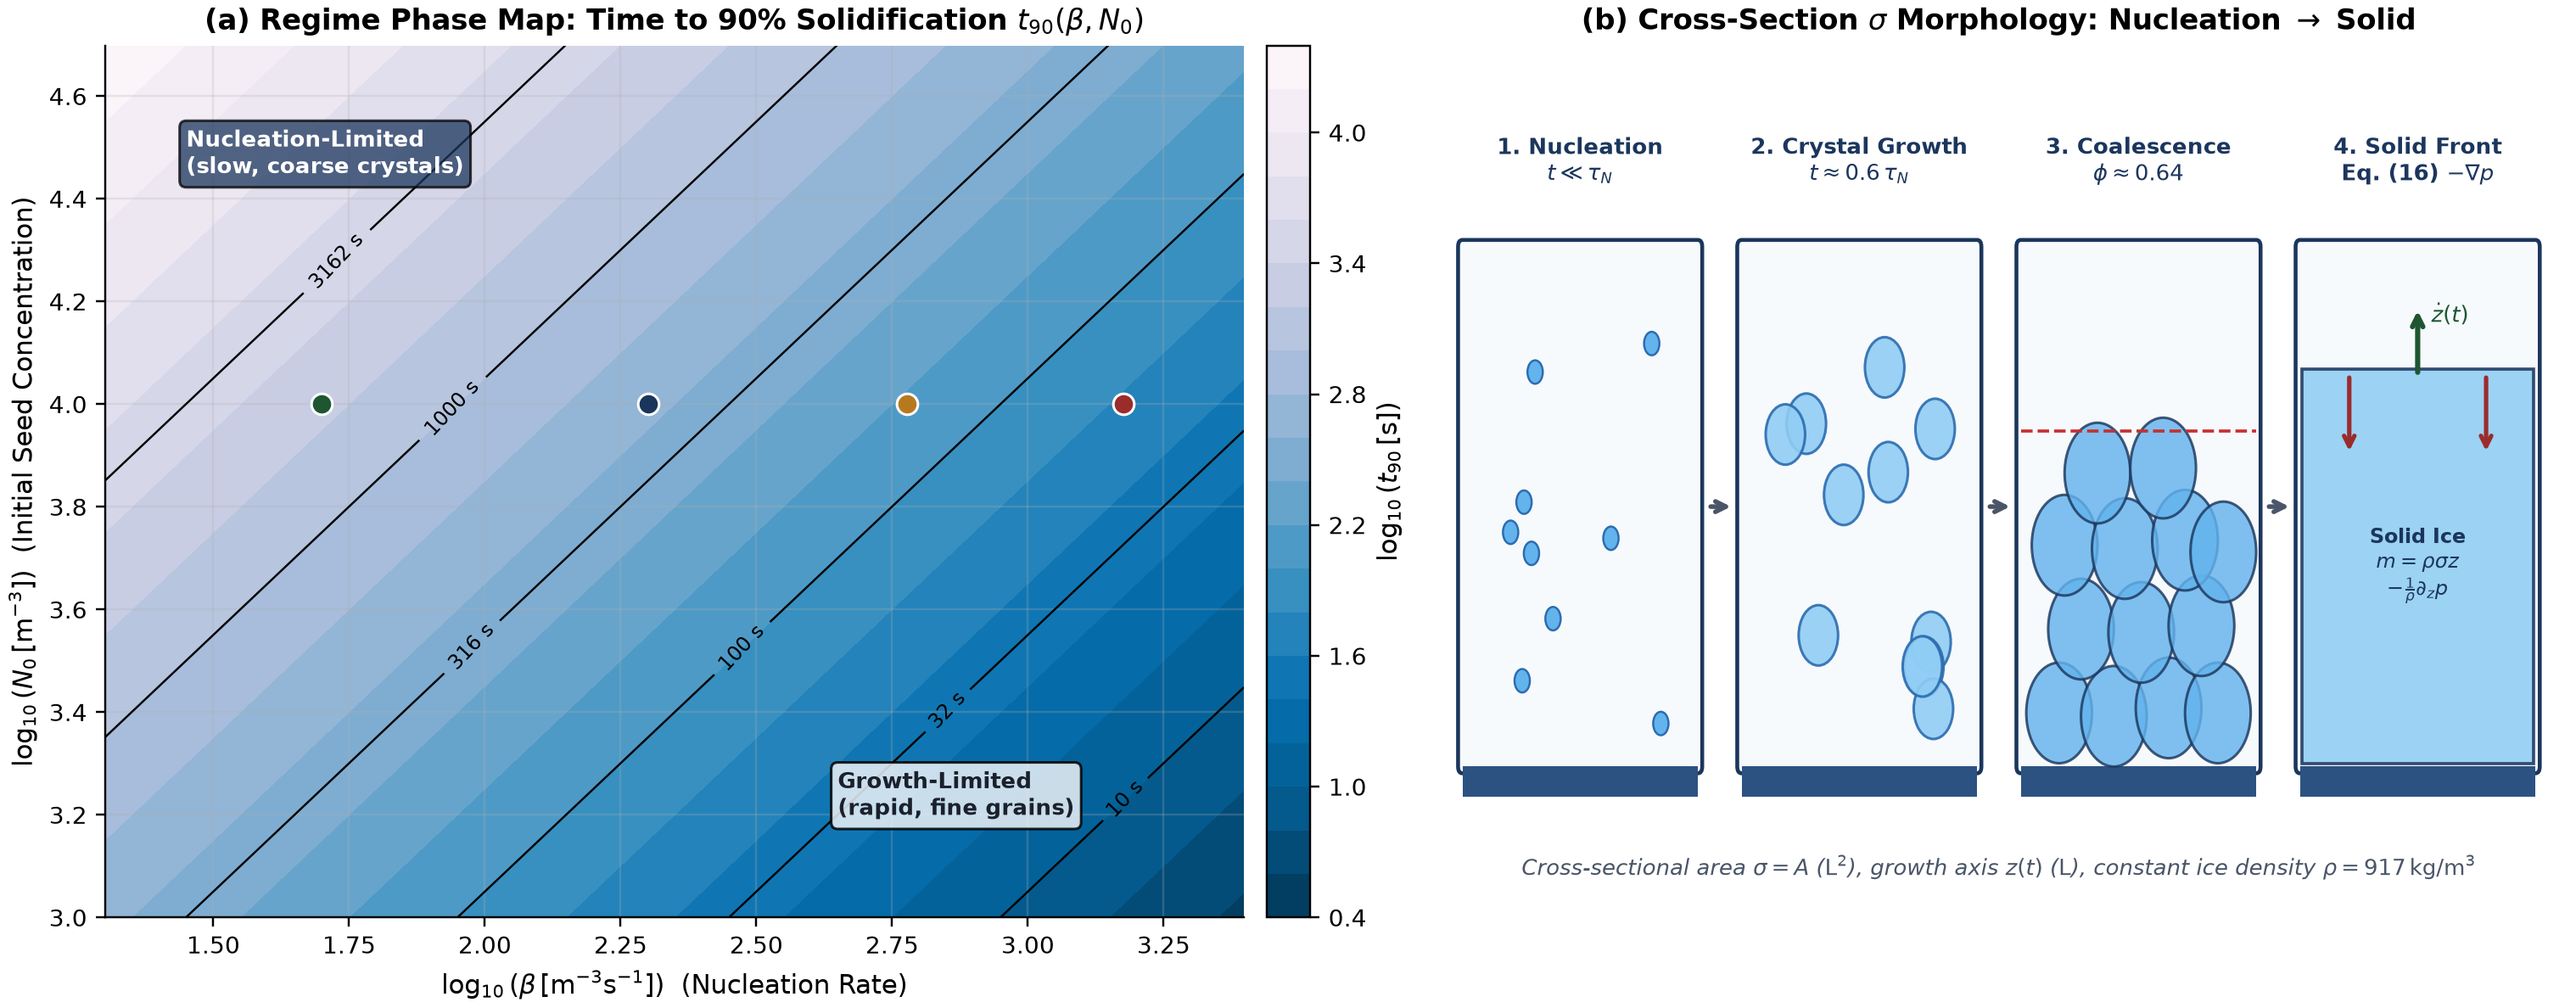
\includegraphics[width=0.98\textwidth]{../../figures/ice_fig3_regime_and_morphology.png}
  \caption{(a)~2D solidification phase map $t_{90}(\beta, N_0)$ separating nucleation-limited (coarse crystals) from growth-limited (fine grains) regimes. (b)~4-stage physical morphology across cross-section $\sigma$ from discrete nuclei to coalesced continuum solid mass.}
  \label{fig:morphology}
\end{figure}

% ============================================================================
\section{Verification \& Conservation Audit (\texttt{rosolver})}
% ============================================================================

\begin{resultbox}{ASME V\&V 20 Verification Summary (\texttt{PASSED})}
\begin{itemize}[leftmargin=1.4em,itemsep=2pt]
  \item \textbf{Analytical Benchmark Verification}: Reference RK4 solve ($\Delta t = 0.5\text{ s}$) matches Eq.~\eqref{eq:z_exact} to $\max|z_{\mathrm{RK4}} - z_{\mathrm{exact}}| = \mathbf{1.68\times 10^{-11}\text{ m}}$ ($\mathrm{RMSE} = 6.97\times 10^{-12}\text{ m}$) and $\max|\dot{z}_{\mathrm{RK4}} - \dot{z}_{\mathrm{exact}}| = \mathbf{2.41\times 10^{-13}\text{ m/s}}$ (\textbf{PASSED}).
  \item \textbf{RK4 Timestep GCI (\texttt{timestep\_study}, $\Delta t \in \{1, 2, 4\}\text{ s}$)}: Monotonic convergence with observed order $\mathbf{p_{\mathrm{obs}} = 4.0672}$ (formal $4.00$) and $\mathrm{GCI}_{\mathrm{fine}}^{21} = \mathbf{1.03\times 10^{-7}\%}$ (\textbf{PASSED}).
  \item \textbf{Dual Conservation Audit (\texttt{audit\_ode\_invariants})}: Both symbolic identities verified exact; discrete drift $\max|m + m_{\mathrm{liq}} - m_{\max}| = \mathbf{7.77\times 10^{-16}\text{ kg}}$ and Eq.~(16) impulse drift $\max|\rho\dot{z} + P_{\mathrm{imp}} - \rho\dot{z}_0| = \mathbf{2.11\times 10^{-15}\text{ Pa}\cdot\text{s/m}}$ (\textbf{PASSED}).
\end{itemize}
\end{resultbox}

\begin{figure}[htbp]
  \centering
  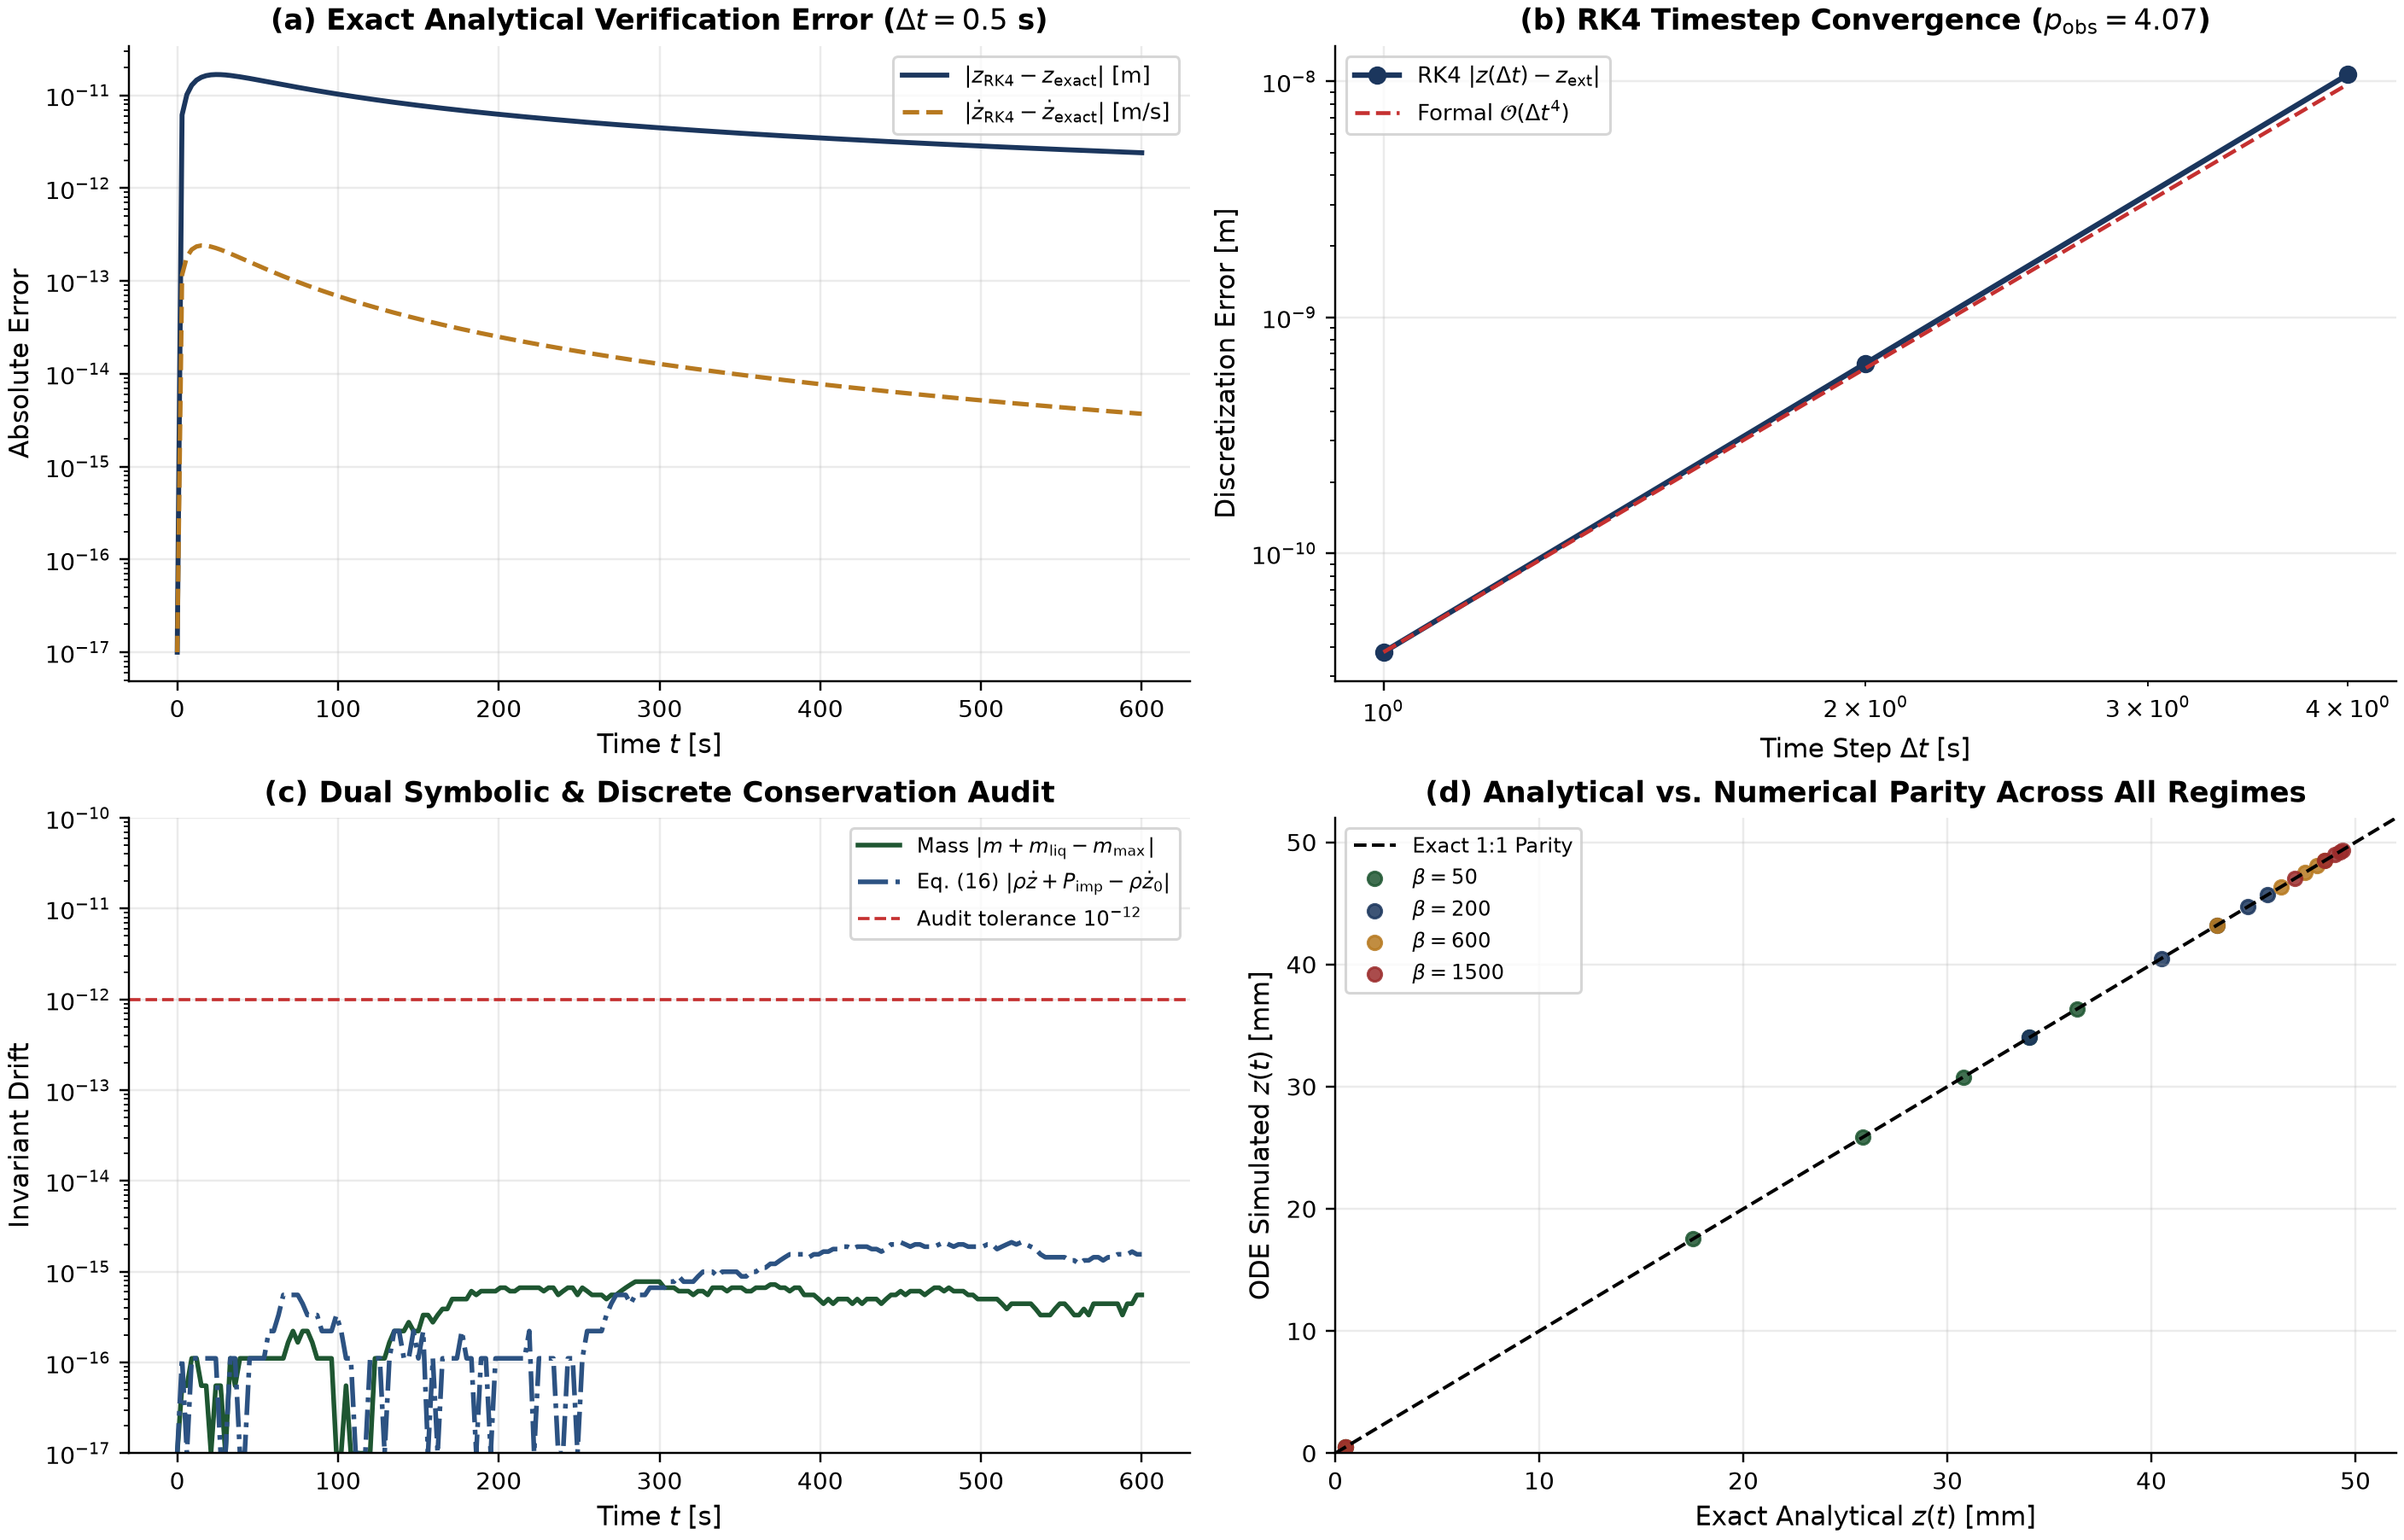
\includegraphics[width=0.96\textwidth]{../../figures/ice_fig4_verification_suite.png}
  \caption{Four-pillar \texttt{rosolver} verification diagnostics: (a)~analytical error vs.\ time, (b)~4th-order RK4 discretization convergence, (c)~dual mass and Eq.~(16) momentum-impulse conservation residuals, and (d)~1:1 parity across all four nucleation regimes.}
  \label{fig:vv}
\end{figure}

\vspace{0.5em}
\noindent\emph{Scope Note}: Verification diagnostics follow ASME V\&V~20-2009 / Roache / Celik engineering traceability practices and do not constitute formal regulatory certification.

\end{document}
